% This is samplepaper.tex, a sample chapter demonstrating the
% LLNCS macro package for Springer Computer Science proceedings;
% Version 2.21 of 2022/01/12
%
\documentclass[runningheads]{llncs}
%
\usepackage[T1]{fontenc}
% T1 fonts will be used to generate the final print and online PDFs,
% so please use T1 fonts in your manuscript whenever possible.
% Other font encondings may result in incorrect characters.
%
\usepackage{graphicx}
\usepackage{algorithm}
\usepackage{algorithmic}
\usepackage{newfloat}
\usepackage{listings}
%\DeclareCaptionStyle{ruled}{labelfont=normalfont,labelsep=colon,strut=off} % DO NOT CHANGE THIS
\lstset{%
	basicstyle={\footnotesize\ttfamily},% footnotesize acceptable for monospace
	numbers=left,numberstyle=\footnotesize,xleftmargin=2em,% show line numbers, remove this entire line if you don't want the numbers.
	aboveskip=0pt,belowskip=0pt,%
	showstringspaces=false,tabsize=2,breaklines=true}
\floatstyle{ruled}
\newfloat{listing}{tb}{lst}{}
\floatname{listing}{Listing}
%
% Keep the \pdfinfo as shown here. There's no need
% for you to add the /Title and /Author tags.
\pdfinfo{
/TemplateVersion (2023.1)
}
\usepackage{amsmath}
\usepackage{amsfonts}
\usepackage{tikz}
\usepackage{multirow}
%\usepackage[usenames,dvipsnames]{color}
\usepackage{color, colortbl}
%\usepackage{url}
\usepackage{bm}
\usepackage{booktabs}
\usepackage{verbatim}
%\usepackage[linesnumbered, boxed, ruled]{algorithm2e}
%
%\usepackage[noend]{algpseudocode}


\usepackage{bbding}
%\usepackage{subfigure}
%\usepackage{caption}
\usepackage{subcaption}
\captionsetup{compatibility=false}
%\captionsetup[sub]{compatibility=false}
%\hypersetup{
%	colorlinks=true,
%	linkcolor=blue
%}

%\newtheorem{example}{Example}
\newcommand{\secref}[1]{Section \ref{#1}}
\newcommand{\figref}[1]{Figure \ref{#1}}
\newcommand{\eqnref}[1]{Eq. (\ref{#1})}
\newcommand{\tabref}[1]{Table \ref{#1}}
\newcommand{\exref}[1]{Example \ref{#1}}
\newcommand{\KZ}[1]{\textcolor{blue}{Kenny: #1}}
\newcommand{\Roy}[1]{\textcolor{red}{Roy: #1}}
\newcommand{\crosssymbol}{{\color{red} \XSolidBrush} }
\newcommand{\checksymbol}{{\color{green} \Checkmark} }
\newcommand{\cut}[1]{}

\usepackage{makecell}

\newcommand\BibTeX{B\textsc{ib}\TeX}
\definecolor{Gray}{gray}{0.9}



\setcounter{secnumdepth}{0} %May be changed to 1 or 2 if section numbers are desired.



\title{Reducing Short Circuits in Multiple-Choice Natural Language Reasoning Models with Data Augmentation}

%Example, Single Author, ->> remove \iffalse,\fi and place them surrounding AAAI title to use it
\iffalse
\author {
    Author Name
}
\affiliations{
    Affiliation\\
    Affiliation Line 2\\
    name@example.com
}
\fi

\iffalse
%Example, Multiple Authors, ->> remove \iffalse,\fi and place them surrounding AAAI title to use it
\title{My Publication Title --- Multiple Authors}
\author {
    % Authors
    First Author Name,\textsuperscript{\rm 1}
    Second Author Name, \textsuperscript{\rm 2}
    Third Author Name \textsuperscript{\rm 1}
}
\affiliations {
    % Affiliations
    \textsuperscript{\rm 1} Affiliation 1\\
    \textsuperscript{\rm 2} Affiliation 2\\
    firstAuthor@affiliation1.com, secondAuthor@affilation2.com, thirdAuthor@affiliation1.com
}
\fi


\appendix
\begin{document}


\section{A.  Details of Stress Tests}
\tabref{tab:results} tells more detailed numbers
\footnote{The dashes in \tabref{tab:results} are caused by limited test cases 
which sizes are too small.} 
about 
stress test results with different aspects in Figure 4. (Section 3.2)
%(\secref{sec:fine-grained})
%\KZ{Use refs to main text here!}

\begin{table*}[th]
\scriptsize
\centering
\begin{tabular}{ll|c|ccccccc}\hline
\toprule  
\textbf{Dataset}&\textbf{Model}&\textbf{Original} &\textbf{Neg+} & \textbf{Neg-} &\textbf{NER} &\textbf{PR} &\textbf{PI}&\textbf{Voice}&\textbf{All}
                                               \\ 
 \hline
 \multirow{15}{*}{ROC} 
&BT(w/o)&88.49 &80.24 &60.99 &84.90 &78.47 &89.47 &60.26 &77.48 \\ 
&BT+B&88.42 &86.99 &68.79 &86.00 &82.76 &88.97 &68.02 &82.35 \\ 
&BT+C&87.60 &80.73 &62.76 &99.63 &91.42 &99.03 &72.52 &85.35 \\ 
&BT+M&87.69 &78.36 &85.10 &93.37 &87.64 &95.39 &95.50 &87.60 \\ 
&BT+C+M&87.47 &82.99 &81.91 &99.17 &93.60 &98.92 &95.23 &91.31 \\ 
\cline{2-10}
&XL(w/o)&90.88 &86.94 &60.99 &88.03 &52.50 &94.00 &52.76 &73.95 \\ 
&XL+B&90.88 &87.39 &57.09 &92.36 &53.99 &96.44 &54.08 &75.30 \\ 
&XL+C&90.52 &88.65 &57.09 &99.45 &89.03 &99.30 &61.47 &85.38 \\ 
&XL+M&90.08 &86.98 &76.60 &94.29 &70.92 &97.29 &98.88 &88.02 \\ 
&XL+C+M&90.40 &85.61 &81.21 &99.35 &91.71 &99.62 &97.37 &92.35 \\ 
\cline{2-10}
&RB(w/o)&92.16 &87.50 &61.35 &77.62 &65.99 &88.97 &64.10 &77.58 \\ 
&RB+B&92.16 &88.56 &64.89 &77.99 &61.91 &90.05 &57.89 &76.17 \\ 
&RB+C&91.68 &88.24 &70.57 &99.63 &92.36 &98.68 &73.70 &88.46 \\ 
&RB+M&91.91 &87.96 &81.56 &95.21 &71.36 &96.28 &99.48 &88.55 \\ 
&RB+C+M&92.46 &87.67 &82.62 &99.72 &96.02 &99.61 &99.34 &94.39 \\ 
\hline
\multirow{15}{*}{COPA} 
&BT(w/o)&64.60 &56.44 &-&-&69.41 &74.89 &53.93 &62.55 \\ 
&BT+B&75.40 &73.22 &-&-&85.16 &71.54 &80.49 &77.47 \\ 
&BT+C&75.73 &69.69 &-&-&91.87 &77.02 &70.60 &76.94 \\ 
&BT+M&69.53 &74.66 &-&-&82.01 &81.43 &97.29 &82.19 \\ 
&BT+C+M&73.20 &77.97 &-&-&92.48 &86.30 &96.47 &86.83 \\ 
\cline{2-10}
&XL(w/o)&63.40 &58.53 &-&-&55.59 &78.54 &64.77 &62.47 \\ 
&XL+B&64.80 &69.90 &-&-&58.74 &79.15 &50.54 &64.81 \\ 
&XL+C&74.60 &73.58 &-&-&91.16 &96.65 &75.34 &82.54 \\ 
&XL+M&66.80 &69.69 &-&-&63.01 &85.84 &99.73 &76.65 \\ 
&XL+C+M&72.93 &84.44 &-&-&89.64 &98.18 &99.86 &91.38 \\ 
\cline{2-10}
&RB(w/o)&72.00 &73.87 &-&-&60.36 &75.65 &64.91 &68.90 \\ 
&RB+B&74.07 &82.51 &-&-&65.44 &82.65 &80.63 &77.71 \\ 
&RB+C&77.07 &88.55 &-&-&94.21 &97.41 &87.94 &91.45 \\ 
&RB+M&70.47 &83.37 &-&-&73.07 &95.74 &99.59 &86.01 \\ 
&RB+C+M&75.67 &86.03 &-&-&95.73 &99.54 &99.86 &93.63 \\ 
\hline
\multirow{15}{*}{ARCT} 
&BT(w/o)&61.94 &11.78 &80.26 &-&52.11 &42.26 &17.43 &33.07 \\ 
&BT+B&71.70 &49.83 &67.10 &-&43.66 &35.72 &19.92 &44.75 \\ 
&BT+C&70.80 &35.13 &83.33 &-&69.48 &77.98 &45.98 &53.87 \\ 
&BT+M&65.92 &42.20 &94.52 &-&84.51 &83.93 &93.48 &71.82 \\ 
&BT+C+M&68.54 &38.94 &95.39 &-&81.69 &92.26 &89.85 &70.22 \\ 
\cline{2-10}
&XL(w/o)&77.85 &43.88 &80.26 &-&41.78 &42.86 &53.45 &53.20 \\ 
&XL+B&77.70 &46.57 &80.92 &-&44.13 &57.14 &46.17 &54.00 \\ 
&XL+C&78.60 &45.68 &81.58 &-&66.20 &84.53 &58.24 &60.71 \\ 
&XL+M&75.45 &44.55 &91.01 &-&62.91 &81.55 &93.10 &69.73 \\ 
&XL+C+M&76.95 &45.68 &93.86 &-&75.59 &95.83 &93.29 &73.07 \\ 
\cline{2-10}
&RB(w/o)&77.10 &36.92 &80.04 &-&46.95 &60.12 &40.61 &49.20 \\ 
&RB+B&80.93 &48.71 &78.73 &-&44.60 &60.71 &40.42 &53.38 \\ 
&RB+C&79.05 &44.89 &83.55 &-&66.67 &80.95 &41.57 &56.71 \\ 
&RB+M&78.23 &52.41 &93.64 &-&68.07 &77.38 &92.14 &73.33 \\ 
&RB+C+M&77.78 &49.05 &92.54 &-&79.34 &95.83 &91.76 &74.13 \\ 
\hline
\multirow{15}{*}{RECLOR} 
&BT(w/o)&45.60 &25.87 &36.13 &-&19.56 &24.91 &13.81 &23.08\\ 
&BT+B&48.60 &28.71 &33.61 &-&26.09 &30.77 &17.24 &26.06\\ 
&BT+C&47.00 &23.64 &48.74 &-&43.12 &53.85 &31.81 &33.94\\ 
&BT+M&46.80 &21.24 &53.78 &-&43.84 &32.60 &50.32 &36.81\\ 
&BT+C+M&43.60 &23.47 &54.90 &-&47.46 &50.92 &47.91 &39.29\\ 
\cline{2-10}
&XL(w/o)&56.00 &30.58 &52.94 &-&32.24 &39.19 &20.28 &31.52\\ 
&XL+B&57.00 &31.29 &43.42 &-&31.16 &43.95 &27.76 &33.05\\ 
&XL+C&54.40 &31.47 &63.87 &-&47.83 &62.27 &34.22 &40.92\\ 
&XL+M&53.60 &29.78 &64.71 &-&50.72 &54.94 &56.65 &46.20\\ 
&XL+C+M&54.20 &30.31 &68.91 &-&55.43 &62.64 &58.18 &48.58\\ 
\cline{2-10}
&RB(w/o)&50.40 &25.33 &48.46 &-&27.53 &38.46 &16.73 &27.34\\ 
&RB+B&51.00 &19.82 &40.62 &-&24.27 &27.10 &8.88 &20.53\\ 
&RB+C&50.40 &30.66 &58.54 &-&46.38 &45.06 &35.74 &38.54\\ 
&RB+M&52.00 &29.96 &60.78 &-&50.73 &43.96 &54.12 &44.01\\ 
&RB+C+M&48.40 &30.22 &64.71 &-&53.99 &57.88 &53.23 &46.03\\ 



\bottomrule
\hline
\end{tabular}
\caption{\label{tab:results} Detailed Breakdown of Stress Tests
on 4 models with or without(w/o) data augmentation. 
+B = augmented with backtranslation,
+C = augmented with crossover, +M = augmented with mutation. 
Stress Tests includes the following stress tests: 
Neg+=negation-add, Neg-=negation-remove, NER, 
PR=pronoun-replacement, PI=Pronoun-instantiation, Adv=adverbial, Voice, Syn=synonym.}
\end{table*}




\section{B.   Details of Choice-only test}
In~\tabref{tab:only-test}, we show specific numbers for Figure 5 which describe 
the choice-only results. (Section 3.3)
%(\secref{sec:choice-only})
\begin{table}[th]
\centering
\scriptsize
\begin{tabular}{c|rrrr}
\toprule
\textbf{Model} & \textbf{ROC} & \textbf{COPA} & \textbf{ARCT} & \textbf{RECLOR} \\ \midrule
BT(w/o)&64.10 &51.67 &59.01 &35.60 \\ \hline  
BT+B&64.90 &55.07 &65.47 &35.13 \\ \hline  
BT+C&59.99 &50.67 &61.71 &28.67 \\ \hline  
BT+M&62.44 &57.53 &59.31 &31.80 \\ \hline  
BT+C+M&60.82 &52.87 &56.38 &30.93 \\ \midrule 
XL(w/o)&73.12 &57.47 &68.09 &35.13 \\ \hline  
XL+B&72.88 &57.67 &67.72 &35.73 \\ \hline  
XL+C&65.01 &59.53 &61.64 &29.53 \\ \hline  
XL+M&71.69 &58.93 &64.41 &35.93 \\ \hline  
XL+C+M&67.72 &58.53 &61.11 &32.00 \\ \midrule 
RB(w/o)&76.23 &60.33 &69.75 &32.60 \\ \hline  
RB+B&74.63 &60.47 &71.10 &38.00 \\ \hline  
RB+C&72.73 &57.33 &67.12 &33.87 \\ \hline  
RB+M&71.28 &54.40 &64.04 &36.53 \\ \hline  
RB+C+M&73.35 &57.40 &65.01 &33.53 \\


%BT (w/o)&54.62&51.4&61.94&42.8 \\ \hline
%BT+B&58.26&50.8&64.41&39.2  \\ \hline
%BT+C&51.2&48.2&55.63&30.8  \\ \hline
%BT+M&51.79&48.8&55.18&38   \\ \hline
%BT+C+M&43.56&49.4&52.03&33.8  \\ \midrule
%XL (w/o)&71.14&57&65.99&42.2 \\ \hline
%XL+B&73.17&60&66.89&41.4  \\ \hline
%XL+C&65.63&55&55.86&34.2  \\ \hline
%XL+M&71.94&57.8&66.22&42  \\ \hline
%XL+C+M&66.22&58.4&62.84&35  \\ \midrule
%RB (w/o)&73.97&59.4&67.79&30.2 \\ \hline
%RB+B&74.77&61.4&69.37&42.2  \\ \hline
%RB+C&73.06&58.4&68.47&34.6  \\ \hline
%RB+M&70.34&56&61.49&40      \\ \hline
%RB+C+M&71.3&54.8&67.79&32.2  \\ 
\bottomrule
\end{tabular}
\caption{Choice-only test for transformer-based models on 4 datasets. All numbers are percentages (\%)}
%\KZ{I assume this is the ending-only test? But isn't smaller the better
%for ending-only tests?}}
\label{tab:only-test}
\end{table}

\section{C.   Extra Cases}
We have shown an example in Section 3.4 
%\secref{sec:case} 
for the case study. In this section of the appendix, we 
provide extra 3 cases for further illustrating that \textit{crossover} and \textit{mutation} 
encourage models to build contextual reasoning  
by attending to relevant concepts in the premise. 
%can better enourage transformer-based models to pay attention to premise and the relationship 
%between premise and choices. 

\begin{example}\label{ex:copa1}
An MCQ from COPA:\\ \\
\noindent
\textbf{Premise:} I pushed the door. \\
\textbf{Choice 1:} The door opened.  \checksymbol  \\
\textbf{Choice 2:} The door locked. \crosssymbol
\end{example}

In \exref{ex:copa1}, we explore RoBERTa-based models by 
analyzing their attention maps on this question in~\figref{fig:case}.  
In this example, the word ``pushed'' in the premise is strongly
related with the word ``opened'' in the right choice from human knowledge. 
The relationship between these two words is the key to answering this question. 
We explore different models with the augmentation method with attention map 
to visualize if these two words have a relationship or not.
%The attention map is visualized via an off-the-shelf tool~\cite{vig-2019-multiscale}.
\begin{figure}[th!]
\centering
\begin{subfigure}[b]{0.40\textwidth}
\centering

\framebox{\includegraphics[width=\columnwidth]{figure/case_original.eps}}
\caption{RB(w/o)}
\label{fig:case_original}
\end{subfigure}
\hfill
\begin{subfigure}[b]{0.40\textwidth}
\centering
\framebox{\includegraphics[width=\columnwidth]{figure/case_b.eps}}
\caption{RB+B}
\label{fig:case_b}
\end{subfigure}
\hfill
\newpage
\begin{subfigure}[b]{0.40\textwidth}
\centering
\framebox{\includegraphics[width=\columnwidth]{figure/case_c.eps}}
\caption{RB+C}
\label{fig:case_c}
\end{subfigure}
\hfill
\begin{subfigure}[b]{0.40\textwidth}
\centering
\framebox{\includegraphics[width=\columnwidth]{figure/case_cm.eps}}
\caption{RB+C+M}
\label{fig:case_cm}
\end{subfigure}
\caption{Attention map on a COPA example for models.}
%\KZ{Caption is wrong! most graphs are fine. 
%But ReCLOR (RB) is a bit strange. 
%Why is BT line exactly the same as the BT+C? And why is BT+B so bad?}}
\label{fig:case}
\end{figure}


In \figref{fig:case}, 
RoBERTa trained on the original training set fails to pick up the 
relation between ``pushed'' and ``opened''. 
After training with \textit{crossover} data augmentation, 
the model learns to build contextual reasoning  
by attending to relevant concepts in the premise. 
Similar trends also exist for the combination of \textit{crossover} 
and \textit{mutation} operation in~\figref{fig:case_cm}. 
These observations empirically demonstrate the effectiveness of our methods 
to encouraging the model to pay attention to the premise so as to improve 
model robustness. On the contrary, back-translation in \figref{fig:case_b} seems 
to have not enhanced such abilities.

\begin{example}\label{ex:copa2}
An MCQ from COPA:\\ \\
\noindent
\textbf{Premise:} I was furious.\\
\textbf{Choice 1:} I slammed the door upon leaving the house.  \checksymbol \\
\textbf{Choice 2:} I checked the mailbox upon leaving the house. \crosssymbol
\end{example}

\begin{figure}[th!]
\centering
\begin{subfigure}[b]{0.40\textwidth}
\centering
\framebox{\includegraphics[width=\columnwidth]{figure/copa2_o.eps}}
\caption{XL(w/o)}
\label{fig:copa2_o}
\end{subfigure}
\hfill
\newpage
\begin{subfigure}[b]{0.40\textwidth}
\centering
\framebox{\includegraphics[width=\columnwidth]{figure/copa2_b.eps}}
\caption{XL+B}
\label{fig:copa2_b}
\end{subfigure}
\hfill
\begin{subfigure}[b]{0.40\textwidth}
\centering
\framebox{\includegraphics[width=\columnwidth]{figure/copa2_c.eps}}
\caption{XL+C}
\label{fig:copa2_c}
\end{subfigure}
\hfill
\newpage
\begin{subfigure}[b]{0.40\textwidth}
\centering
\framebox{\includegraphics[width=\columnwidth]{figure/copa2_m.eps}}
\caption{XL+M}
\label{fig:copa2_m}
\end{subfigure}
\hfill
\begin{subfigure}[b]{0.40\textwidth}
\centering
\framebox{\includegraphics[width=\columnwidth]{figure/copa2_cm.eps}}
\caption{XL+C+M}
\label{fig:copa2_cm}
\end{subfigure}
\caption{Attention map on a COPA example for XLNet-based models.}
%\KZ{Caption is wrong! most graphs are fine. 
%But ReCLOR (RB) is a bit strange. 
%Why is BT line exactly the same as the BT+C? And why is BT+B so bad?}}
\label{fig:copa2_bert}
\end{figure}

In human cognition, the word ``furious'' in premise and ``slammed'' in the right choice 
have a strong causal relationship in~\exref{ex:copa2}. 
However, from the attention map of the vanilla XLNet model in \figref{fig:copa2_bert}, 
it is difficult to observe that they are related. 
In \figref{fig:copa2_bert}, we also observe that 
the ability of XLNet to use relationships has been strengthened by adding augmented data with all 
methods we mentioned. Back-translation is worse than the other methods with lighter color blocks.

\begin{example}\label{ex:arct1}
An MCQ from ARCT:\\ \\
\noindent
\textbf{Premise:} I would be happy to support free community college so those who can't afford it can get educated. College should be free.\\
\textbf{Choice 1:} I would be happy to pay tuition for everyone , even some rich kids.  \checksymbol \\
\textbf{Choice 2:} I would not be happy to pay for some rich kids tuition at the same time. \crosssymbol
\end{example}

\begin{figure}[th!]
\centering
\begin{subfigure}[b]{0.28\textwidth}
\centering
\framebox{\includegraphics[width=\columnwidth]{figure/arct1_o.eps}}
\caption{BT(w/o)}
\label{fig:arct1_o}
\end{subfigure}
\hfill
\newpage
\begin{subfigure}[b]{0.28\textwidth}
\centering
\framebox{\includegraphics[width=\columnwidth]{figure/arct1_b.eps}}
\caption{BT+B}
\label{fig:arct1_b}
\end{subfigure}
\hfill
\begin{subfigure}[b]{0.28\textwidth}
\centering
\framebox{\includegraphics[width=\columnwidth]{figure/arct1_c.eps}}
\caption{BT+C}
\label{fig:arct1_c}
\end{subfigure}
\hfill
\newpage
\begin{subfigure}[b]{0.28\textwidth}
\centering
\framebox{\includegraphics[width=\columnwidth]{figure/arct1_m.eps}}
\caption{BT+M}
\label{fig:arct1_m}
\end{subfigure}
\hfill
\begin{subfigure}[b]{0.28\textwidth}
\centering
\framebox{\includegraphics[width=\columnwidth]{figure/arct1_cm.eps}}
\caption{BT+C+M}
\label{fig:arct1_cm}
\end{subfigure}
\caption{Attention map on an ARCT example for BERT-based models.}
%\KZ{Caption is wrong! most graphs are fine. 
%But ReCLOR (RB) is a bit strange. 
%Why is BT line exactly the same as the BT+C? And why is BT+B so bad?}}
\label{fig:arct1_bert}
\end{figure}

In~\exref{ex:arct1}, the claim and reason are ``College should be free'' and 
``I would be happy to support ... who can't afford it can get educated'' separately. 
The word ``free'' is very important for the claim. 
It should be very related to the information in the correct warrant, 
such as ``tuition'' or ``pay'' from the knowledge of commonsense reasoning. 
Unfortunately, ``free'' has little relationship with the warrant in~\figref{fig:arct1_o}
through the vanilla BERT model. 
Consistent with our previous conclusion, 
the improvement effect of \textit{crossover} and \textit{mutation} 
is more obvious than back-translation. 
Besides, we also observe that the performance of data augmentation methods 
is not as obvious as the first two examples. 
One reason may be that analyzing with this white-box method is not completely reliable. 
The other may be that the ability of these data augmentation methods to reduce short circuits 
and to improve the stability of the model is limited. 
We will continue to study the reason in the future.

\section{D.   Details of Stress Test Human Evaluation} 
We have generated stress test cases with different operators and 
the size of cases have shown in Section 3.1. 
To guarantee the correctness of questions in the stress test, we make 
human annotation by sampling 100 cases from each kind of stress test. 
If the total number of a stress test is less than 100, we will consider all  
cases which have been generated. 
The pass rate for each test is shown in \tabref{tab:pass_rate}. 
Mostly, the test cases are perfect (100 percent pass rate) except for Neg+ stress test cases. 
To make Neg+ test more convincing, we annotate all generated 
Neg+ cases and filter the Neg+ stress test cases from 492 cases to 463 cases. 
All models are tested on this human filtered test set. 
\begin{table}[th]
\centering
\scriptsize
\begin{tabular}{c|rrrr}
\toprule
\textbf{Stress} & \textbf{ROC} & \textbf{COPA} & \textbf{ARCT} & \textbf{RECLOR} \\ \midrule
Neg+  & 100&94&  100&100 \\ \hline
Neg-  & 100& -&  100&    100\\ \hline
NER  &  100&    -&  -&- \\ \hline
PR  &   100&100&100&100   \\ \hline
PI  &        100&   100&    100& 100\\  \hline
Voice  &    100&100   &100    &100    \\  \bottomrule
%Adv  & 1,850&496   &444    &500    \\ \hline
%CO  &  1,871&500   &444    &500    \\ \hline
%Syn&   653&     25&    303&289 \\ \midrule
%MT  &  1,871&500   &444    &500    \\ \hline
%Total & 11,446  &  2,808 & 2,390 & 2,709 \\ \bottomrule
\end{tabular}
\caption{Pass rate (\%) of stress test cases with human annotation.}
\label{tab:pass_rate}
\end{table}

\end{document}
